\documentclass{article}
\usepackage{graphicx}
\title{Reading Journal}
\author{Henry Oehlrich}

\begin{document}

\maketitle{}

\subsection{Wed Nov 16 | The C Programming Language}
\textit{Page started: 46 \\
        Page ended: 62 \\
        Time: 1 hour
        Content: Rather technical bits \\
}

I chose to read \textit{The C Programming Language} by Dennis Ritchie and Brian
Kerninghan. Among programming languages, C is considered one of the most
classic and esoteric. It is a statically typed, compiled language, with low
level control over memory, and is incredibly dangerous. C's close proximity to
the hardware makes it both exceptionally powerful as well as dangerous
(proponents of C call this "efficiently dangerous"). While I usually prefer to
learn languages from experience and more hands on things, I made an exception
for this book. The authors, Dennis Ritchie and Brian Kerninghan are near
deities in the world of *nix computing and some denominations of computer
science. Ritchie wrote C himself (with minor assistance from Kerninghan) as a
successor to the B programming language (created by Ken Thompson). C was
developed in the early 70's as a higher level (meaning a higher level of
abstraction from the hardware) alternative to assembly. Up until that point
(with the exception of Fortran) almost all programming was done in assembly.
Assembly is basically just a more human-readable for of machine code, with just
a few simple instructions that had to be manipulated in a way to do what you
wanted. Assembly was not a language so much as a class of languages. Each
processor architecture (or type) had it's own incompatible assembly language.
This made code highly importable, you had to rewrite it just to move it to a
different type of machine. C, on the other hand is compiled, meaning that
another program (also written in C - its kinda funky how that works) takes what
you have written, and converts it into the assembly language for the processor
that you are running. This means that you "merely" must write a C compiler for
each architecture of CPU you want. And then, you can use each of those
compilers to compile programs for multiple architectures without having to
rewrite. Note: this is an incredibly high level and oversimplified version of
how a compiler works, it is actually much more difficult to do this. As a
whole, C's syntax is easy. There are a minimal amount of keywords (compared to
other languages), and there are few external functions. This simplicity is
deceiving: the reason it looks simple is because it forces you to write a bunch
of stuff from scratch. Many features that are taken for granted in more
popular, larger languages simply don't exist in C's standard library (nor can
you easily install external libraries). This is one of the main reasons I'd
like to learn it. I've probably written far to much... I'm going to stop now.

\subsection{Wed Nov 21 | The Fellowship of the Ring - The Ring Goes South}
\textit{Page started: 1 \\
        Page ended: 42 \\
        Time: 1 hour \\
}

I took a break from the other more technical book to come back to the Lord of
the Rings. I understand that I am supposed to be reading something new and this
is not a new book for me. But, I am reading it in a different light :). For
fear of merely reiterating the, might a say wonderful, plot, I was going to
write about the dichotomy and hierarchy of Tolkien's works. The Lord of the
Rings was originally pitched to Tolkien's publisher, Allen and Unwin, as a
immediate successor to the Hobbit. The Hobbit was a short children's story
written in the world that the Professor had been creating over the previous
years. Fast-forward several years and you have the Lord of the Rings. Tolkien
imagined The Lord of the Rings as a single novel with six sections (or as he
called them: books); intended to be read from start to finish. His publisher,
on the other hand, not wanting to commit to a multi-thousand page publication
demanded that he separate the novel into more reasonably sized chunks. Tolkien
reluctantly split his novel into three volumes, with each volume having two
books. The Fellowship of The Ring contained The Ring Sets Out and The Ring Goes
South. The Two Towers contained The Treason of Isengard and The Ring Goes East.
The Return of the King contained The War of the Ring and The End of the Third
Age. The Lord of the Rings, much to the Professor's disgruntlement, is
erroneously called a trilogy when it is in fact a single novel. The naming of
the volumes was also a matter of dispute between Tolkien and his publishers.
Tolkien simply wanted to name the books: The Lord of The Rings vol 1, vol 2,
and vol 3. Allen and Unwin virtually created the names of the books that we
attribute to Tolkien. The Professor himself said that the titles of the volumes
were too flashy and gave away too much of the plot. He seems to have a point
with at least The Return of the King. Tolkien's Legundarium does not end at
the Lord of the Rings. A majority of the information we know about Middle Earth
was published post-mortem (I believe that means what I think it means). After
his death, his son, Christopher Tolkien compiled all of the Professor's notes
into one, concise, simple book. The man himself had been trying to do this for
over three decades. The difficulty in this task arose because of the vast
disorganization of the material. Most of what went down on paper was hastily
scrawled and unordered. Not to mention that there were hundreds of conflicting
versions of stories and characters, all of which created by one person. In fact,
to get a grasp on how much information was created, it might be easier for one
to know that a thirteen-book explanation on the creation of Middle Earth, was
written. Christopher Tolkien wrote The History of Middle Earth as not a history
of the world, but rather a history of the creation of the world. It contains
much of the versioning and writing process. I've probably written far to
much... I'm going to stop now.

\subsection{Wed Nov 28 | The Fellowship of the Ring - The Ring Goes South}
\textit{Page started: 42 \\
        Page ended: 253 (end) \\
        Time: many hours \\
}

Over Thanksgiving break, I finished the second volume of the Lord of the Rings.
It was the second part of Fellowship, starting at their arrival at Imladris
(Rivendell) and ending with the departure of Sam and Frodo and the death of
Boromir. Given that this is not the first time I've read this, I made a point
of spending more time on the poems and songs scattered throughout the book.
Many of these poems (while published before the Silmarillion) rely on the
history and information layed out in the Silmarillion. My favorite was 

\pagebreak{}
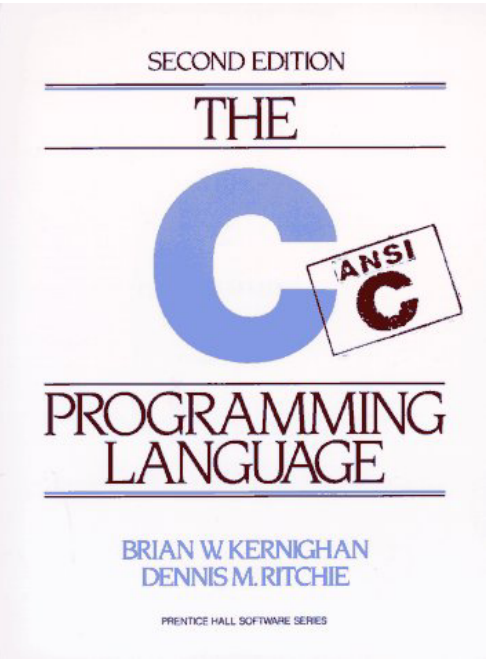
\includegraphics[width=\textwidth]{images/the-c-programming-language.png}
\end{document}
